\documentclass[12pt,a4paper]{article}
\usepackage{clrscode}
\usepackage[conEntregas]{tp2}
\usepackage[spanish]{babel} % para que comandos como \today den el resultado en castellano
\usepackage{a4wide} % márgenes un poco más anchos que lo usual
\usepackage[T1]{fontenc}
\usepackage{textcomp}
\usepackage{graphicx}
\usepackage{enumitem}
\newcommand{\subscript}[2]{$#1 _ #2$}
\usepackage[utf8]{inputenc} 
\usepackage{pdfpages}
\usepackage{amsmath}
\usepackage{vmargin}
\setpapersize{A4}


\begin{document}
\titulo{Trabajo Práctico 2}
\subtitulo{Modelando problemas problemas con grafos}

\fecha{\today}

\materia{Algoritmos y Estructura de Datos III}

\integrante{Buceta, Diego}{001/17}{diegobuceta35@gmail.com}
\integrante{Springhart, Gonzalo}{318/17}{glspringhart@gmail.com}
% Pongan cuantos integrantes quieran

\maketitle

\newpage
%\includepdf[pages={1,2}]{tp1.pdf}

\section{Introducción al problema}
\section{Justificación teórica}
\section{Algoritmos presentados}
\subsection{Kruskal}
\begin{codebox}
  \Procname{$\proc{KruskalSinPathComp}(ListaIncidencia: grafoCompleto, cantNodos: entero)$}
\li padre $\gets$ vector de enteros de tamaño de cantNodos y cargado con el valor de su posición en cada posición
\li AGM $\gets$ lista de incidencia vacia, de tamaño cantNodos-1
\li OrdenarPorPeso(grafoCompleto)
\li \For e:Arista $\in$ grafoCompleto 
\li \If $getPadre(indice(e.primerNodo), padre) $=$ getPadre(indice(e.segundoNodo),padre)$ \Then
\li agregar(e,agm)
\li \End
\li \End
\li Devolver AGM
\end{codebox}

\begin{codebox}
\Procname{$\proc{getPadre}(entero: indice, padre: vector de enteros)$}
\li \If $padre[indice] == indice$ \Then
\li Devolver indice
\li \Else
\li getPadre(indice(padre[indice]),padre)
\li \End
\end{codebox}


\begin{codebox}
\Procname{$\proc{getPadreConPathComp}(entero: indice, padre: vector de enteros, altura:vector de enteros, nivelesSubidos: entero$}
\li \If $padre[indice] == indice$ \Then
\li altura[indice] = nivelesSubidos
\li Devolver indice
\li \Else
\li padre[indice] = getPadreConPathComp(indice(padre[indice]),padre,altura,nivelesSubidos+1)
\li Devolver padre[indice]
\li \End
\end{codebox}


\begin{codebox}
\Procname{$\proc{unirPadres}(indiceNodo1: entero, indiceNodo2:entero, padre: vector de enteros)$}
\li padreNodo1 $\gets$ getPadre(indiceNodo1, padre)
\li padre[indiceNodo2]=padreNodo1
\end{codebox}

\begin{codebox}
\Procname{$\proc{unirPadresConPathComp}(indiceNodo1: entero, indiceNodo2:entero, padre: vector de enteros, altura:vector de enteros, nivelesSubidos: entero)$}
\li padreNodo1 $\gets$ getPadreConPathComp(indiceNodo1, padre,altura,0)
\li padreNodo2 $\gets$ getPadreConPathComp(indiceNodo2, padre,altura,0)
\li padreMenosAltura $\gets$ min(altura[padreNodo1],altura[padreNodo2])
\li padreMasAltura $\gets$ max(altura[padreNodo1],altura[padreNodo2])
\li padre[padreMenosAltura]=padreMasAltura
\end{codebox}


\begin{codebox}
\Procname{$\proc{armarGrafoCompleto}(nodos:vector de Nodos)$}
\li listaAristas $\gets$ inicializar lista de incidencia
\li matrizAristas $\gets$ inicializar matriz de adyacencia
\li \For $i \gets 0$ \To $tam(nodos)$
\li 	\For  $j \gets i+1$ \To $tam(nodos)$
			\li armar arista con datos de v[i] y v[j]
			\li agregar arista a listaAristas
		\End
	\End
\li armar matriz de adyacencia con la lista de incidencia
\li Devolver Matriz de adyacencia y Lista de incidencia
\end{codebox}

\begin{codebox}
\Procname{$\proc{retirarEjesInconsistentes}(listaAristas:lista incidencia, \sigma_{T}, profVecindario, f_{T}, forma, cantidadDeClusters, padre: vector de enteros )$}
\li \For $e:listaAristas$
\li calcular media y desviacion respecto del vecindario de profVecindario de profundidad de cada extremo de e. (usando una modificación de BFS)
\li si es inconsistente
\li sacar e de las listas
\li recorrer en la lista de ady todos los nodos alcanzables de uno de los extremos y modificar su representante en padre con cantidadDeClusters (usando una modificación de BFS)
\li aumentar en 1 el valor de cantidadDeClusters

\li \End
\end{codebox}


\subsection{Complejidad}

\section{Experimentación}
\subsection{Variaciones}
\begin{verse}
Tomaremos los casos de test brindados en http://cs.joensuu.fi/sipu/datasets/ y correremos nuestro algoritmo para poder obtener las clusterizaciones.\\
Los experimentos estarán centrados en analizar las diferentes tipos clusterizaciones que pueden realizarse variando las definiciones de eje inconsistente. Intentaremos analizar las configuraciones necesarias para que se pueda alcanzar una clusterización lo más cercana a la de la percepción humana y los resultados interesantes al que pueden llegarse.

Dados los siguientes: $f_{T}$ multiplicador del promedio, $\sigma_{T}$ multiplicador de la desviación, y la profundidad del vecindario de los extremos del eje candidato, W(XY) el peso del eje candidato, y sea X e Y sus nodos extremos, definiremos un eje inconsistente:
\begin{itemize}
\item Forma 1: $\frac{W(XY)}{Promedio(Vecindario(X))}$ $>$ $f_{T}$ $  y $ $\frac{W(XY)}{Promedio(Vecindario(Y))}$ $>$ $f_{T}$, \\Es decir, la proporción entre el peso del eje candidato y el promedio de peso del vecindario de sus extremos es mayor al coeficiente dado.
\item Forma 2: $W(XY) >  Promedio(Vecindario(X)) + \sigma_{T}$ $ * $ $ desviacion(Vecindario(X)) $ $ y$ $W(XY) >  Promedio(Vecindario(Y)) + \sigma_{T}$ $ * $ $ desviacion(Vecindario(Y)) $, \\Es decir, que el peso del eje candidato supere al promedio del vecindario de sus extremos por al menos $\sigma_{T}$ unidades de la desviación del vecindario del extremo.
\item Forma 3: Que se cumpla ambas
\end{itemize}


Comencemos señalizando que la clusterización no es un problema matemáticamente definido y por ello podemos definirlo de forma tal que se obtenga diferentes resultados para mismas situaciones. 
La clusterización es la organización y detección de patrones en nuestros datos en grupos que tengan algún significado. Por lo general, a partir de un lote de datos, se busca caracterizarlos en base a la información que se pueda obtener de ellos y no por un patrón o clase de datos conocida dada. Es decir, no se separan los datos en función de su característica en propiedades o atributos previamente fijados, sino que se evalúa la correlación de cada uno de ellos entre todos los datos y en función de esto se agrupan. Estos analisis suelen dividirse como analisis supervisado y no supervisados (o clusteing), donde en los supervisados se cuenta inicialmente con las caracterizaciones que se esperan obtener y se analizan los datos para el reconocimiento de los patrones que permitan situarlo en el modelo correcto. Algunos ejemplos son redes neuronales, árboles de decisión, etc. Discutir el significado de correlación y significancia depende en gran medida de la naturaleza de los datos que se organicen. En nuestro caso, tenemos datos númericos correspondientes a puntos en el plano y en donde vamos a tomar como relación primaria entre ellos como su distancia euclídea. Experimentaremos con casos ya conocidos de clusterización y evualuaremos fuertemente la habilidad del modelo y sus parámetros para acercarse a los resultados de nuestra percepción, aunque siempre teniendo en mente la literatura del problema de clusterización y particularmente los analisis de los principios de agrupación propuestos por la filosofía de Gestalt previamente analizados.\\


\begin{center}
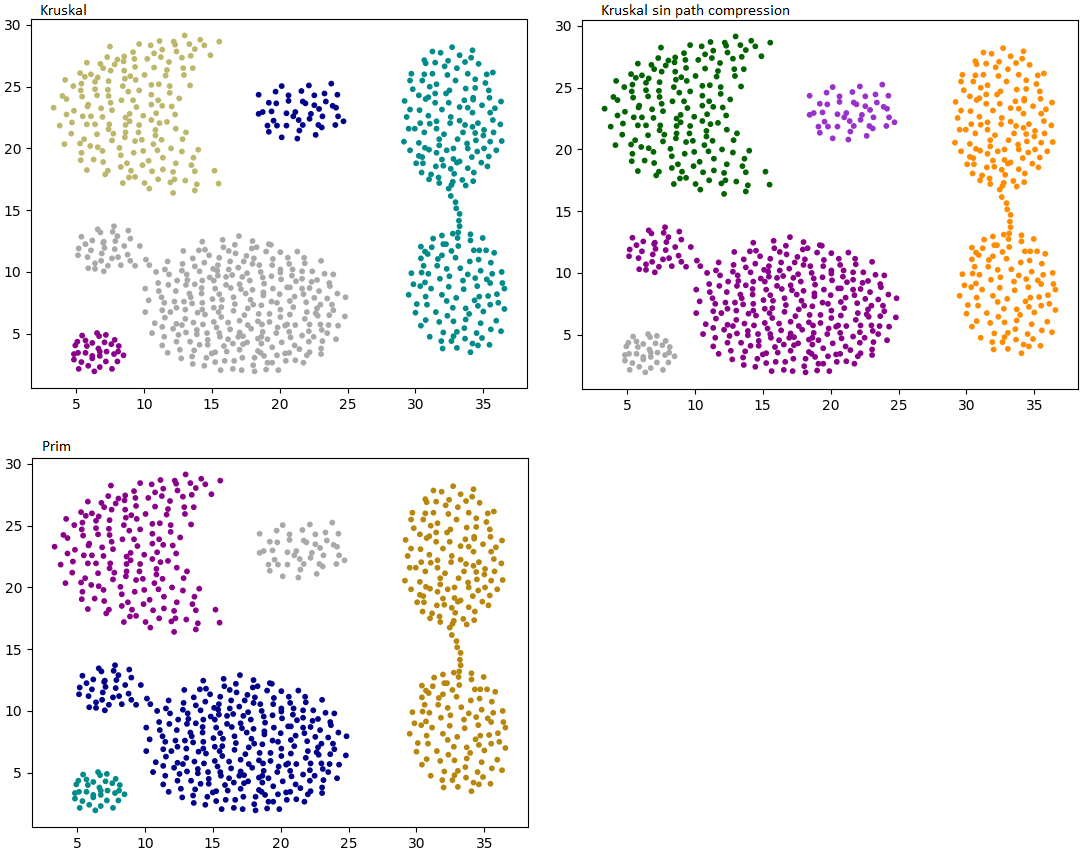
\includegraphics[scale=.4]{graficos/aggregation.png}
\end{center}

Analizando el siguiente caso podemos ver que generando el AGM con cualquiera de los métodos elegidos obtenemos la misma clusterización. Elegimos como parámetros que un eje inconsistente debe superar en 2.5 al promedio de los vecinos de 2 pasos de sus extremos. La clasificación resulta en 5 clusters. Como primera observación, la percepción humana podría arrojar que el cluster de la esquina derecha en realidad podrían ser dos clusters diferentes, al igual que el cluster de la esquina izquierda. Si intentamos conseguir algo más cercano a esto, podemos intentar clasificar ahora también teniendo en cuenta la desviación. Como todos los puntos tienen una densidad de vecinos parecida, no tiene mucho sentido modificar la distancia del vecindario de los extremos (actualmente dos). Si reducimos el coeficiente del promedio de 2.5 hasta 1.4 y el coeficiente de la desviación lo fijamos en 2. Después de varios intentemos, encontramos que en ese punto obtenemos lo siguiente:


\begin{center}
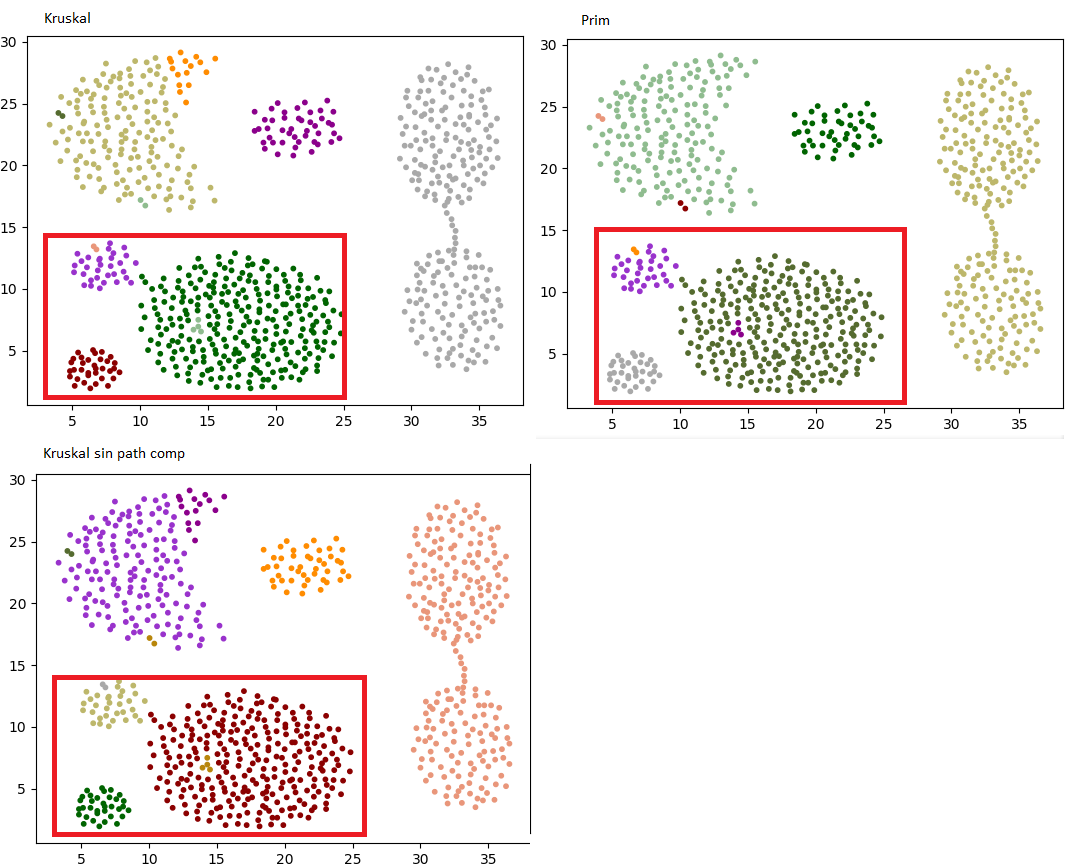
\includegraphics[scale=.4]{graficos/aggregation2.png}
\end{center}
\end{verse}

Por un lado, conseguimos aumentar los clusters. Sin embargo, las modificaciones que hagamos para dividir clusters anteriores resultan en divisiones no deseadas en otros que ya estaban 'bien' según nuestra percepción. Ahora pudimos encontrar una forma de clusterizar más parecida a nuestra percepción el cluster señalado. Sin embargo, esto produce ciertas inconsistencias. Por ejemplo, poder identificar más de un grupo nos cuesta encontrar ahora cuatro. Excepto en kruskal con path compression, en los otros dos encontramos un mini-cluster dentro del cluster grande marcado con rojo, a su ve también el nuevo cluster ahora en turquesa dentro de la marcación tiene también un mini-cluster. En los demás fuera de la marca también encontramos este tipo de cosas. Podríamos pensar entonces que en este tipo de situaciones en donde hay grandes grupos de cluster bien definidos y las densidades de puntos similares en cada uno, podemos fácilmente clasificarlos de forma similar a nuestra percepción. Sin embargo, cuando queremos perfeccionarlo, nos encontramos con dificultades para poder seguir manteniendo la consistencia en los demás clusters. \\
Una posible solución a esto podría ser hacer un 'zoom' a la zona de clusters que nos interesa. De esa forma conseguiríamos abstraernos de la clasificación de los demás y centrarnos sólo en los que nos interesa.\\
Entonces una de las cosas que vamos a ver es si esto es realmente factible y entonces podemos utilizar esta técnica para poder ver a grandes rasgos los clusters y en función de nuestro interes enfocarnos en una zona en particular. Esto nos facilita porque al momento de volver a clasificar esa zona, lo haríamos restringiendo nuestro domino de patrones (anteriormente de todo el conjunto de puntos) hacia uno más pequeño.\\ 

\end{document}
